\begin{figure}[ht]
\centerline{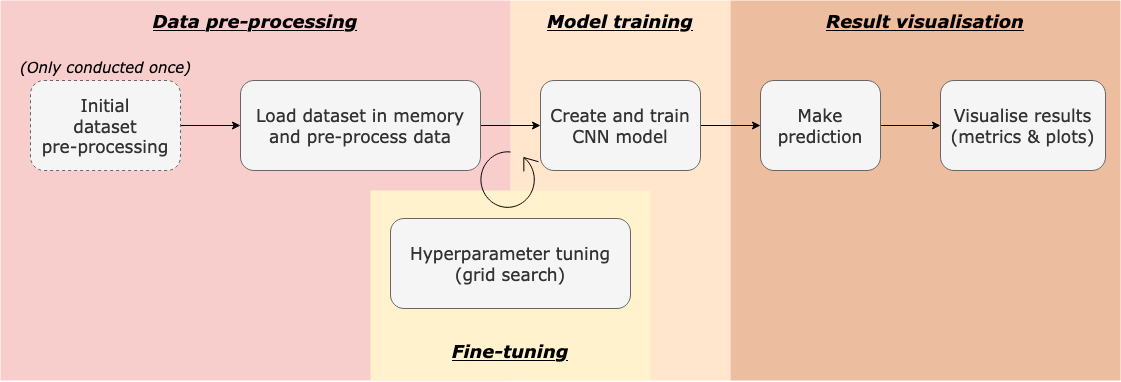
\includegraphics[width=1.1\textwidth]{Dissertation/figures/design/design flowchart.png}}
\caption{\label{fig:design-flowchart}Flowchart. Created using draw.io.}
\end{figure}

\section{Dataset \& Classification type}

An early design decision taken as a group consisted in which datasets to use. The small size of mini-MIAS dataset  

Why choose CBIS-DDSM over DDSM? Binary classification vs multi-class classification.\\

CBIS-DDSM uses uncompressed images (DICOM vs LJPEG - which is no longer used), meaning they can be fed into the CNN with larger sizes, allowing the model to learn more high-level features.

\section{Deep Learning Pipeline Design Analysis}

\subsection{Dataset pre-processing}

\subsubsection{Processing and organising raw images}

File formats: PGM and DICOM files need to be converted.

\subsubsection{Data loading}

The mini-MIAS dataset is very small in size (339 Mb before pre-processing, 202 Mb after pre-processing), containing only 322 images. It can therefore be loaded into memory without any data loading optimisation techniques. However, the CBIS-DDSM dataset is much larger, containing 10,239 images that cover 163.6 Gb of disk space. The dataset therefore cannot be loaded in memory in a single import and needs to be loaded in batches.\\ % mention batches and caching

\subsection{CNN Model}

\subsubsection{Training}

One-hot encoding of labels (for both binary and multi-class classification).\\

Training/testing/validation split using stratified and shuffling splits (keep class balance and reorder images in directories).\\

CNN models with pre-trained weights on ImageNet to avoid training from scratch. However, this  forces the input images to have the same size as the images in ImageNet it was trained on.\\

Early stopping conditions.\\

\subsubsection{Testing}

todo

\subsection{Output}

Output metrics chosen: a combination of numerical metrics and visual metrics.


\begin{itemize}
    \item numerical metrics:
    \begin{itemize}
        \item overall accuracy
        \item precision
        \item recall
        \item F1 score
    \end{itemize}
    \item visual metrics:
    \begin{itemize}
        \item confusion matrix
        \item normalised confusion matrix
        \item Receiver Operating Characteristic (ROC) curve
    \end{itemize}
\end{itemize}

%%%%%%%%%%%%%%%%%%%%%%%%%%%%%%%%%%%%%%%%%%%%%%%%%%%%%%%%%%%%%%%%%%%%
%%%%%%%%%%%%%%%%%%%%%%%%%%%%%%%%%%%%%%%%%%%%%%%%%%%%%%%%%%%%%%%%%%%%
%%%%%%%%%%%%%%%%%%%%%%%%%%%%%%%%%%%%%%%%%%%%%%%%%%%%%%%%%%%%%%%%%%%%

\section{General Design Decisions}

\subsection{Programming Language}

Choosing a programming language is one of the most essential aspect to take into account as it is the medium used to transform the system from design to implementation. However, choosing from over 250 different programming languages \cite{tiobe} can be tricky, which is why multiple views have to be evaluated before choosing a programming language. Four popular programming languages are considered for this project: Python, Java, R and  Javascript.\\

The first element to consider is the availability of third-party libraries used for implementing common machine learning methods, as well as data pre-processing, manipulation and visualisation techniques found in deep learning systems to avoid manually implementing them. The most popular libraries nowadays consist of Tensorflow (which is available in Python, R and Javascript) and PyTorch (which is available in Python). Additionally, Compute Unified Device Architecture (CUDA) support for GPU optimisations, CNN support and pre-trained models need to be included for the implementation of the desired deep learning breast cancer detection system, which are available in all libraries.\\

In terms of speed, compiled languages are quicker than interpreted languages. However, the main bottleneck in a deep learning system is the training phase of the model, which mainly relies on the library used rather than the language itself. Therefore, speed is not taken into account. Finally, of all the programming languages mentioned, Python is the favoured one in terms of personal preference, familiarity, and experience, especially when applied to machine learning implementations. Therefore, the wide support for machine learning libraries in Python, coupled with the personal preference for the language, make Python the obvious programming language candidate for this project.\\

For a complete review of the main pros and cons considered between when deciding between Python, Java, R and Javascript, refer to Appendix~\ref{ch:appendix-programming_languages_comparison}.

\subsection{Deep Learning Framework}

To complete. Justify Tensorflow/Keras over PyTorch.

\subsection{Interface}

A Command-Line Interface (CLI) is selected, allowing arguments and flags to be passed to execute different sections of the code. Arguments control the dataset to use, the CNN model, and the mode to run in (training or testing). Flags control the verbose mode to print more statements in the terminal for debugging purposed. The full set of instructions to run the code can be found in Appendix~\ref{ch:appendix-usage-instructions}.
